\documentclass[varwidth=6.2in,border=3pt]{standalone}
\usepackage{tikz}
\usetikzlibrary{arrows.meta,decorations.pathreplacing,positioning,calc,fit}
\usepackage{amsmath}
\usepackage{algpseudocode}
\usepackage{newtxtext,newtxmath}
\newcommand{\code}[1]{\texttt{#1}}
\newcommand{\truesum}{\code{truesum}}
\begin{document}
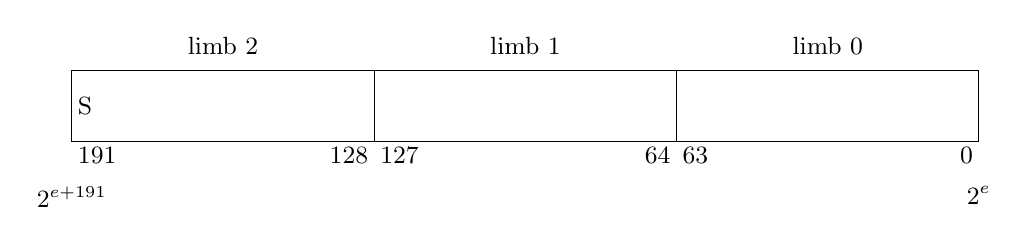
\begin{tikzpicture}[x=0.06cm,y=0.9cm,font=\small]
  % Most significant limb on the left, so each limb runs high bit to low bit.
  \foreach \k/\hi/\lo in {2/191/128,1/127/64,0/63/0} {
    \pgfmathsetmacro{\x}{(2-\k)*64}
    \draw (\x,0) rectangle (\x+64,1);
    \node at (\x+32,1.35) {limb \k};
    \node[anchor=north west,inner sep=2pt] at (\x,0) {\hi};
    \node[anchor=north east,inner sep=2pt] at (\x+64,0) {\lo};
  }
  \node[anchor=west,inner sep=2pt] at (0,0.5) {S};
  \node[anchor=north] at (0,-0.5) {$2^{e+191}$};
  \node[anchor=north] at (192,-0.5) {$2^{e}$};
\end{tikzpicture}
\end{document}
